\documentclass[11pt]{exam}
\input{../../Header/packages.sty}
\input{../../Header/styleExam.sty}
\input{../../Header/headerQuestion.sty}
\input{../../Header/mathexpressions.sty}
\graphicspath{{data-algebra/}}
%=========================================================
\newcommand{\theme}{Logarithmus}
\newcommand{\teacher}{Jonas Guler}
%=========================================================
\begin{document}
\fontsize{14}{14}\selectfont
\begin{center}
    \huge\bf\theme
\end{center}

\begin{questions}
%=========================================================
%-------------------TESTFRAGEN
%=========================================================
\noaddpoints
\question[\totalpoints]
\addpoints
\begin{parts}
    \part[2] Beschreibe in eigenen Worten, was ein Logarithmus ist und inwiefern er mit der Exponentialfunktion verbunden ist.
    \part[1] Erkläre einem Laien in zwei Sätzen, den Unterschied zwischen einer Polynomialgleichung und einer Exponentialgleichung. Veranschauliche deine Erklärung mit einem passenden Beispiel.
\end{parts}
\begin{parts}
    \setcounter{partno}{2}
    \part[2] Welcher der folgenden Ausdrücke passt nicht dazu? Begründe deine Antwort.
    \[\log{4}{2}\quad\log{10}{0.01}\quad\log{2}{\frac{1}{8}}\quad\log{3}{\frac{1}{81}}\]
    \part Welcher der folgenden Ausdrücke passt nicht dazu? Begründe deine Antwort.
    \[\log{4}{2}\quad\log{10}{100}\quad\log{2}{8}\quad\log{3}{81}\]
\end{parts}

\begin{parts}
    \setcounter{partno}{4}
    \part[4] Löse die folgende Exponentialgleichung ohne Verwendung des Taschenrechners nach $x$ auf.
    \[7^{2x-1}\*343^{3x+5}=49^{2x-1}\]
    \begin{small}
        Bewertung: Lösungen ohne Lösungsweg ergeben keine Punkte.
    \end{small}
\end{parts}
\begin{parts}
    \setcounter{partno}{5}
    \part[4] Löse die folgende Exponentialgleichung ohne Verwendung von \flqq solve\frqq\: nach $x$ auf. \[5^{x+2}\*125^{2-x}=25^x\]
    \begin{small}
        Bewertung: Lösungen ohne Lösungsweg ergeben keine Punkte.
    \end{small}
\end{parts}
\begin{parts}
	\setcounter{partno}{6}
	\part[4] Löse die folgende Exponentialgleichung ohne Verwendung von \flqq solve\frqq\: nach $x$ auf. \[4^{x-7}\*16^{2x+1}=64^{x+2}\]
	\begin{small}
		Bewertung: Lösungen ohne Lösungsweg ergeben keine Punkte.
	\end{small}
\end{parts}
\begin{parts}
	\setcounter{partno}{7}
	\part[4] Löse die folgende Exponentialgleichung ohne Verwendung von \flqq solve\frqq\: nach $x$ auf. \[3^{2x-1}\*\left(\frac{1}{9}\right)^{7-x}=\left(\sqrt[4]{3}\right)^x\]
	\begin{small}
		Bewertung: Lösungen ohne Lösungsweg ergeben keine Punkte.
	\end{small}
\end{parts}


%---------------------------------------------------------
\question[4]
Welche der folgenden Ausdrücke ist wahr? Begründe deine Antwort.
\begin{parcols}[2]
    \part $\log{10}{11^a}=a$
    \part $\log{b}{\frac{1}{x}}=-\log{b}{x}$
    \part $\log{a}{b}=\frac{\ln{a}}{\ln{b}}$
    \part $\log{2}{x}+\log{3}{y}=\log{2}{x\*y}$
\end{parcols}

\question[4]
Begründe, welche der folgenden Ausdrücke wahr sind und korrigiere die falschen Aussagen.
\begin{parcols}[2]
    \part $\log{a}{u+v}=\log{a}{u}+\log{a}{v}$
    \part $\log{a}{u-v}=\frac{\log{a}{u}}{\log{a}{v}}$
    \part $\log{2}{x}+\log{3}{y}=\log{2}{xy}$
    \part $\log{a}{b}=\frac{\ln{a}}{\ln{b}}$
\end{parcols}

\question[4]
Begründe, welche der folgenden Ausdrücke wahr sind und korrigiere die falschen Aussagen.
\begin{parcols}[2]
    \part $\log{a}{u+v}=\log{a}{u}+\log{a}{v}$
    \part $\log{a}{\frac{u}{v}}=\frac{\log{a}{u}}{\log{a}{v}}$
    \part $\log{2}{x}+\log{3}{y}=\log{2}{xy}$
    \part $\log{a}{c\*u}=c\*\log{a}{u}$
\end{parcols}

\question[4]
In das leere Feld ist jeweils ein Ausdruck so einzufüllen, dass insgesamt eine gültige Aussage entsteht.
\begin{parts}
	\part $\ds\log{a}{\gap{3}}=2\*\log{a}{p}-3\*\log{a}{q}-4\*\log{a}{r}$\\
	\part $\ds\log{a}{\sqrt[3]{q^4}}=\gap{3}\*\log{a}{q}$\\
	\part $\ds\log{a}{a^{-\frac{9}{13}}}=\gap{3}$\\
	\part $\ds\gap{3}=\frac{3\*\ln{x}}{\ln{4}}$\\
\end{parts}


%---------------------------------------------------------
\question[6]
Schreibe den folgenden Logarithmus in möglichst viele Summanden aus.
\begin{parcols}[3]
    \part $\log{a}{5a^2c^3}$
    \part $\log{a}{\frac{2(p^2+q^2)}{x+y}}$
    \part $\log{a}{\frac{\sqrt[3]{u}}{a^5}}$
\end{parcols}

%---------------------------------------------------------
\question[2]
Schreibe den folgenden Logarithmus in möglichst viele Summanden aus.
\[\log{m}{\frac{m^2\sqrt[3]{m^2\*\sqrt{n^3}}}{m\*\sqrt[6]{n}}}\]

%---------------------------------------------------------
\question[2]
Schreibe den folgenden Logarithmus in möglichst viele Summanden aus. \[\log{a}{\frac{4\sqrt[3]{x}}{5\sqrt{a^3}}}\]

%---------------------------------------------------------
\question[2]
Schreibe den folgenden Logarithmus in möglichst viele Summanden aus. \[\log{a}{\frac{a^2\sqrt{x}}{x+y}}\]


%---------------------------------------------------------
\question[6]
Fasse den Term zu einem Logarithmus zusammen und vereinfache so weit wie möglich.
\begin{parts}
    \part $\frac{1}{4}\log{3}{81}+\frac{1}{3}\log{2}{8}$
    \part $\log{a}{b^2}+\log{a}{c^2}-\log{a}{b}-\log{a}{c}$
    \part $\ln{x+1}+\ln{x-1}-\ln{x^2-1}$
\end{parts}

%---------------------------------------------------------
\question[2]
Fasse den Term zu einem Logarithmus zusammen und vereinfache so weit wie möglich.
\[\ln{x+1}+\ln{x-1}-\ln{x^2-1}\]

%---------------------------------------------------------
\question[2]
Fasse den Term zu einem Logarithmus zusammen und vereinfache so weit wie möglich.
\[\frac{1}{2}\*\ln{a^{2n}}-(n+2)\ln{a}\]

%---------------------------------------------------------
\question[2]
Fasse den Term zu einem Logarithmus zusammen und vereinfache so weit wie möglich. \[5\*\ln{x+2}-\frac{1}{5}\*\ln{x-2}-4\*\ln{x+2}-\frac{4}{5}\*\ln{x-2}\]


%---------------------------------------------------------
\question[4]
Löse die folgende Gleichung nach $x$ auf. \[\log{x^3}+2\log{x^2}=7\]


%---------------------------------------------------------
\question[4]
Claudia will diese Gleichung lösen: \[5^x=0.2^{3x}\*\exp{x-1}.\] Sie wendet den natürlichen Logarithmus auf beiden Seiten an und erhält \[x\*\ln{5}=3x\*\ln{0.2}\*(x-1).\] Hat sie alles richtig gemacht?
\begin{itemize}
	\item Falls JA, löse die Gleichung fertig.
	\item Falls NEIN, erkläre den Fehler und löse die Gleichung vollständig korrekt.
\end{itemize}


%---------------------------------------------------------
\question[3]
\begin{minipage}{0.6\linewidth}
    Im Koordinatensystem sind drei Graphen von Logarithmusfunktionen eingezeichnet. Ordne die drei Graphen ihrer Funktionsgleichung zu.
    \begin{parts}\begin{multicols}{2}
        \part $y=\log{\frac{1}{3}}{x}$
        \part $y=\log{2}{x-1}$
        \part $y=\log{2}{x}+2$
        \part $y=\log{\frac{1}{2}}{x}$
        \part $y=\log{2}{x+1}$
        \part $y=\log{2}{x-1}+2$
    \end{multicols}\end{parts}
\end{minipage}
\hfill
\begin{minipage}{0.35\linewidth}
    \centering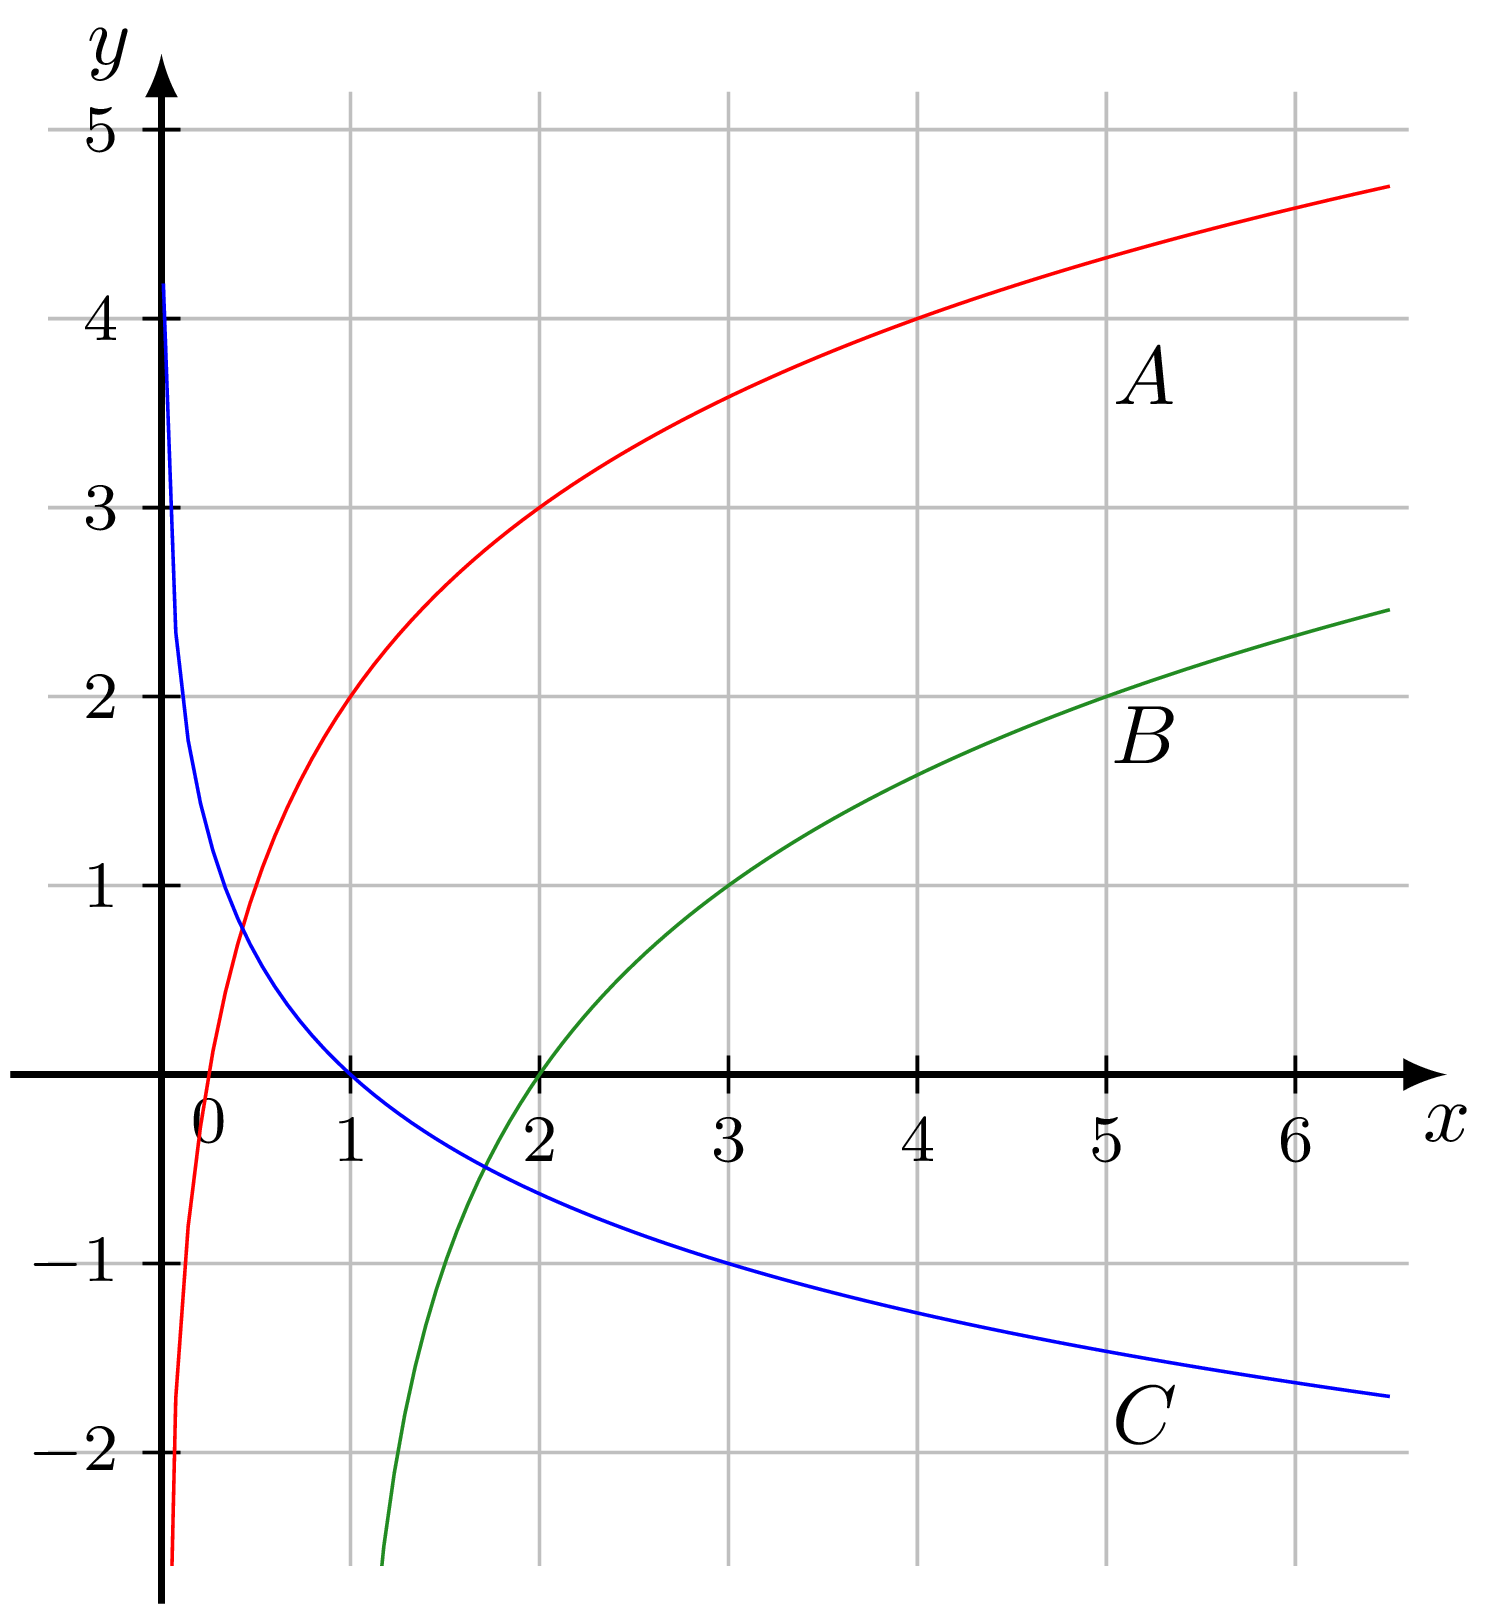
\includegraphics[scale=0.1]{data-algebra/LogGraphen2.png}
\end{minipage}

%---------------------------------------------------------
\question[8]
Berechne die folgenden Logarithmen mithilfe des kleinen Taschenrechner. Notiere deinen Lösungsweg und markiere darin, wo du den Taschenrechner zur Hilfe genommen hast.
\begin{parts}
    \begin{multicols}{2}
        \part $\log{4}{12}$
        \part $3\*\log{e}{10}$
        \part $\log{4}{\sqrt{5}}$
        \part $4\cdot\log{9}{3}$
    \end{multicols}
\end{parts}

%---------------------------------------------------------
\noaddpoints
\question[\totalpoints]
\addpoints
\begin{minipage}{0.6\linewidth}
    \begin{parts}
        \part[2] Gezeichnet sind drei Graphen von Funktionen der Form $y=\log{b}{x}$. Gib an welcher zur Funktion mit der kleinsten und welcher zur Funktion mit der grössten Basis $b$ gehört.
        \part[1] Gib die Basis der Funktion des Graphen $\textcolor{red}{B}$ an.
    \end{parts}
\end{minipage}
\hfill
\begin{minipage}{0.375\linewidth}
    \centering
    \begin{tikzpicture}[cross/.style={draw, cross out, minimum size=2*(#1-1pt), inner sep=0pt, outer sep=0pt}, x=10mm, y=10mm, >=latex,   %Voreinstellung für Pfeilspitzen
    	font= \footnotesize, scale=0.9]
    	%Raster zeichnen
    	\draw [color=gray!50]  [step=10mm] (-.3,-2.3) grid (5.3,2.3);
    	% Achsen zeichnen
    	\draw[->,thick] (-.3,0) -- (5.8,0) node[right, below] {\normalsize $x$};
    	\draw[->,thick] (0,-2.3) -- (0,2.8) node[above, left] {\normalsize $y$};
    	% Achsen beschriften
    	\foreach \x in {1,2,...,5} \draw (\x,-.1) -- (\x,.1) node[below=4pt] {$\x$};
    	\foreach \y in {-2,-1,1,2} \draw (-.1,\y) -- (.1,\y) node[left=4pt] {$\y$};
    	% Besserer Ursprung
    	\draw[color=black] (0pt,-7pt) node[left] {$0$};
    	%Funktionen zeichnen:
    	\clip(-.3,-2.3) rectangle (5.8,2.3); %Bildbereich
    	\draw[plotblue, thick, domain=0.01:5.3, samples=100] plot (\x,{ln(\x)/ln(1/2)}) node[above] {$A$};
    	\draw[red, thick, domain=0.01:5.3, samples=100] plot (\x,{ln(\x)/ln(3)}) node[below] {$B$};
    	\draw[forestgreen, thick, domain=0.01:5.3, samples=100] plot (\x,{ln(\x)/ln(2)}) node[below] {$C$};
    \end{tikzpicture}
\end{minipage}

%---------------------------------------------------------
\noaddpoints
\question[\totalpoints]
\addpoints
\begin{minipage}{0.6\linewidth}
    \begin{parts}
        \part[2] Gezeichnet sind drei Graphen von Funktionen der Form $y=\log{b}{x}$. Gib an welcher zur Funktion mit der kleinsten und welcher zur Funktion mit der grössten Basis $b$ gehört.
        \part[1] Gib die Basis der Funktion des Graphen $\textcolor{forestgreen}{A}$ an.
    \end{parts}
\end{minipage}
\hfill
\begin{minipage}{0.375\linewidth}
	\centering
	\begin{tikzpicture}[cross/.style={draw, cross out, minimum size=2*(#1-1pt), inner sep=0pt, outer sep=0pt}, x=10mm, y=10mm, >=latex,   %Voreinstellung für Pfeilspitzen
		font= \footnotesize, scale=0.9]
		%Raster zeichnen
		\draw [color=gray!50]  [step=10mm] (-.3,-2.3) grid (5.3,2.3);
		% Achsen zeichnen
		\draw[->,thick] (-.3,0) -- (5.8,0) node[right, below] {\normalsize $x$};
		\draw[->,thick] (0,-2.3) -- (0,2.8) node[above, left] {\normalsize $y$};
		% Achsen beschriften
		\foreach \x in {1,2,...,5} \draw (\x,-.1) -- (\x,.1) node[below=4pt] {$\x$};
		\foreach \y in {-2,-1,1,2} \draw (-.1,\y) -- (.1,\y) node[left=4pt] {$\y$};
		% Besserer Ursprung
		\draw[color=black] (0pt,-7pt) node[left] {$0$};
		%Funktionen zeichnen:
		\clip(-.3,-2.3) rectangle (5.8,2.3); %Bildbereich
		\draw[plotblue, thick, domain=0.01:5.3, samples=100] plot (\x,{ln(\x)/ln(1/2)}) node[above] {$A$};
		\draw[red, thick, domain=0.01:5.3, samples=100] plot (\x,{ln(\x)/ln(3)}) node[below] {$B$};
		\draw[forestgreen, thick, domain=0.01:5.3, samples=100] plot (\x,{ln(\x)/ln(2)}) node[below] {$C$};
	\end{tikzpicture}
\end{minipage}


%---------------------------------------------------------
\noaddpoints
\question[\totalpoints]
\addpoints
\begin{minipage}{0.6\linewidth}
	\begin{parts}
		\part[2] Gezeichnet sind drei Graphen von Funktionen der Form $y=\log{b}{x}$. Gib an welcher zur Funktion mit der kleinsten und welcher zur Funktion mit der grössten Basis $b$ gehört.
		\part[1] Gib die Basis der Funktion des Graphen $\textcolor{plotblue}{A}$ an.
	\end{parts}
\end{minipage}
\hfill
\begin{minipage}{0.375\linewidth}
	\centering
	\begin{tikzpicture}[cross/.style={draw, cross out, minimum size=2*(#1-1pt), inner sep=0pt, outer sep=0pt}, x=10mm, y=10mm, >=latex,   %Voreinstellung für Pfeilspitzen
		font= \footnotesize, scale=0.9]
		%Raster zeichnen
		\draw [color=gray!50]  [step=10mm] (-.3,-2.3) grid (5.3,2.3);
		% Achsen zeichnen
		\draw[->,thick] (-.3,0) -- (5.8,0) node[right, below] {\normalsize $x$};
		\draw[->,thick] (0,-2.3) -- (0,2.8) node[above, left] {\normalsize $y$};
		% Achsen beschriften
		\foreach \x in {1,2,...,5} \draw (\x,-.1) -- (\x,.1) node[below=4pt] {$\x$};
		\foreach \y in {-2,-1,1,2} \draw (-.1,\y) -- (.1,\y) node[left=4pt] {$\y$};
		% Besserer Ursprung
		\draw[color=black] (0pt,-7pt) node[left] {$0$};
		%Funktionen zeichnen:
		\clip(-.3,-2.3) rectangle (5.8,2.3); %Bildbereich
		\draw[plotblue, thick, domain=0.01:5.3, samples=100] plot (\x,{ln(\x)/ln(1/3)}) node[above] {$A$};
		\draw[red, thick, domain=0.01:5.3, samples=100] plot (\x,{ln(\x)/ln(2)}) node[below] {$B$};
		\draw[forestgreen, thick, domain=0.01:5.3, samples=100] plot (\x,{ln(\x)/ln(5)}) node[above] {$C$};
	\end{tikzpicture}
\end{minipage}


%---------------------------------------------------------
\question[3]
\begin{minipage}{0.6\linewidth}
    Im Koordinatensystem sind drei Graphen von Logarithmusfunktionen der Form ${f(x)=\log{a}{x}}$ eingezeichnet. Gib die drei Funktionsgleichungen an.
\end{minipage}
\hfill
\begin{minipage}{0.375\linewidth}
    \centering
    \begin{tikzpicture}[cross/.style={draw, cross out, minimum size=2*(#1-1pt), inner sep=0pt, outer sep=0pt}, x=10mm, y=10mm, >=latex,   %Voreinstellung für Pfeilspitzen
    	font= \footnotesize, scale=0.9]
    	%Raster zeichnen
    	\draw [color=gray!50]  [step=10mm] (-.3,-2.3) grid (5.3,2.3);
    	% Achsen zeichnen
    	\draw[->,thick] (-.3,0) -- (5.8,0) node[right, below] {\normalsize $x$};
    	\draw[->,thick] (0,-2.3) -- (0,2.8) node[above, left] {\normalsize $y$};
    	% Achsen beschriften
    	\foreach \x in {1,2,...,5} \draw (\x,-.1) -- (\x,.1) node[below=4pt] {$\x$};
    	\foreach \y in {-2,-1,1,2} \draw (-.1,\y) -- (.1,\y) node[left=4pt] {$\y$};
    	% Besserer Ursprung
    	\draw[color=black] (0pt,-7pt) node[left] {$0$};
    	%Funktionen zeichnen:
    	\clip(-.3,-2.3) rectangle (5.8,2.3); %Bildbereich
    	\draw[plotblue, thick, domain=0.01:5.3, samples=100] plot (\x,{ln(\x)/ln(1/2)}) node[above] {$A$};
    	\draw[red, thick, domain=0.01:5.3, samples=100] plot (\x,{ln(\x)/ln(3)}) node[below] {$B$};
    	\draw[forestgreen, thick, domain=0.01:5.3, samples=100] plot (\x,{ln(\x)/ln(2)}) node[below] {$C$};
    \end{tikzpicture}
\end{minipage}

%---------------------------------------------------------
\noaddpoints
\question[\totalpoints]
\addpoints
Salmonellen sind Bakterien, die schwere Magen-Darm Erkrankungen auslösen. Bei Temperaturen von über $8^\circ$C vermehren sich Salmonellen exponentiell. Die infektiöse Dosis beträgt ca. eine Million Keime.\\ Bei einem infizierten Ei werden um 10:00 Uhr $1000$ Keime gezählt, um 12:00 Uhr sind es bereits $5500$.
\begin{parts}
    \part[1] Gib eine Funktion an, mit welcher sich die Anzahl Keime nach $t$ Stunden ausgehend von 10:00 Uhr berechnen lässt.
    \part[1] Bestimme die Zeit, in der sich die Keimzahl verdoppelt?
    \part[3] Um 16:00 Uhr wird das Ei in ein Kühlfach mit $12^\circ$C gelegt. Das bewirkt, dass sich die Verdopplungszeit\footnote{Die Verdopplungszeit bezeichnet die Zeitspanne, nach der sich der Bestand einer exponentiell wachsende Grösse verdoppelt hat.} vervierfacht. Berechne, um welche Uhrzeit die infektiöse Dosis an Keimen erreicht ist.
\end{parts}

%---------------------------------------------------------
\question[4]
Löse die folgende Gleichung ohne Verwendung von \flqq solve\frqq\:nach $x$ auf. \[\log{2}{x}=1+\log{4}{x}\]
\begin{small}
    Bewertung: Lösungen ohne Lösungsweg ergeben keine Punkte.
\end{small}

%---------------------------------------------------------
\question[4]
Löse die folgende Gleichung ohne Verwendung von \flqq solve\frqq\: nach $x$ auf. \[\log{3}{x-2}=\log{9}{x}\]
\begin{small}
    Bewertung: Lösungen ohne Lösungsweg ergeben keine Punkte.
\end{small}

%---------------------------------------------------------
\question[4]
Löse die folgende Gleichung ohne Verwendung des Taschenrechners nach $x$ auf. \[\log{x}{7x-10}=2\]
\begin{small}
    Bewertung: Lösungen ohne Lösungsweg ergeben keine Punkte.
\end{small}

%---------------------------------------------------------
\question[4]
{\bf Bewertung:} Diese Aufgabe ist ohne Taschenrechner zu lösen.\\
Löse die folgende Gleichung für eine beliebige Basis $a$ nach $x$ auf. \[\log{a}{x^2-5}+\log{a}{x+5}=\log{a}{x+5}\] {\textit{Tipp: Forme die Gleichung sinnvoll mithilfe der Logarithmusgesetzen um.}}


%---------------------------------------------------------
\question[2]
Entscheide in der Tabelle unten, ob die Aussagen wahr oder falsch sind. Die Antworten müssen nicht begründet werden.\newline
\begin{small}
    Bewertung: Für $0-2$ korrekte Antworten gibt es keine Punkte; $3$ korrekte Antworten einen Punkt und falls alle Antworten korrekt sind, gibt es $2$ Punkte.
\end{small}
\begin{table}[h]
    \centering
    \begin{tabular}{|p{12cm}|c|c|}\hline
         & wahr & falsch \\\hline
        Der Logarithmus ist eine alternative Darstellung eines Exponent. & & \\\hline
        Polynomialgleichungen können mithilfe des Logarithmus gelöst werden. & & \\\hline
        Durch geeignetes Logarithmieren kann eine Multiplikation in eine Summe vereinfacht werden. & & \\\hline
        Die Definitions- und Wertemenge sind für die Exponentialfunktion und die Logarithmusfunktion exakt die Gleichen. & & \\\hline
        Durch geeignetes Logarithmieren kann eine Multiplikation in eine Division vereinfacht werden. & & \\\hline
        Exponentialgleichungen können mithilfe des Logarithmus gelöst werden. & & \\\hline
        Der Logarithmus ist eine alternative Darstellung eines Potenz. & & \\\hline
    \end{tabular}
\end{table}


\end{questions}
\end{document}